
\section{General notes}

\subsection{Running the codes - general rules}
The various program executables are to be run in command mode in the Linux/Unix environment. Each command contains the name of the executable file followed by various options. The options are recognized by being preceded by two minus symbols \verb"--". The program options can be of two kinds: pairs specifying the option followed by the value of the option, of the form [option-name  value], or flags. The values can be numbers or strings (arrays of characters). The flags are (boolean) switch signaling that a certain action must occur and do not take any value after them. The general syntax to run a program is:
\begin{verbatim} 
    program_name [--option1 val1] [--option2 val2] [...] [--flag1] [...] 
\end{verbatim}
Running \verb"program_name" without any options sends a manual page to the screen listing the available flags and options with explanations. 

With some exceptions the order of the options and flags in a command does not matter. The specification of certain options is essential for the unambiguous definition of a run, while others are specified only as needed. If any one of the essential options is absent from the command line, the program will warn the user of the missing option and abort.  If the same option is accidentally present multiple times in the command line the last specification is the one that takes effect. 

An alternative way to present options to a program is through an options file \verb"program_name.options".  Each line in this text file contains \verb"option-name : value" pairs separated by a colon. Flags are specified by themselves on separate lines. Note that the command line options take precedence over options supplied  in an \verb".options" file. Examples of such \verb".options" files are provided in the \verb"samples" directory.

The output of the code is typically saved in text files that are column based. The file names are fixed (hard-coded) and, hopefully, suggestive of their content. All output is saved in the directory from which the run command is given. Unless otherwise specified, signal amplitudes are relative to a reference unit amplitude at 1 km. In all cases pressures scaled by the square root of density, $\rho^{-\frac{1}{2}}p$, are written to files rather than the pressure itself. 

\subsection{Atmospheric specifications}
\label{sec: AtmoSpecs}
Necessary input to all propagation codes in this package is the specification of the state of the atmosphere through which propagation is to be modelled. To provide portability and maximum flexibility to the user the state of the atmosphere is input in column-based text files to be provided by the user. Each such file specifies a stratified atmosphere and contains columns such as pressure, density, temperature and the three wind components u, v and w as a function of altitude. Since the vertical wind component w is not used by most of the algorithms its specification is optional. The column order is indicated to the program with the option \verb"--atmosfileorder" followed by a string of characters specifying the order of the columns in the file. For example the profile file may have 7 columns in the order \verb"zuvwtdp":  
\begin{verbatim}
    z - altitude [ km above Mean Sea Level (MSL) ]
    u - West-to-East wind speed [ m/s ]
    v - South-to-North wind speed [ m/s ]
    w - vertical wind (usually zero) [ m/s ]
    t - temperature [ Kelvin ]
    d - density [ g/cm^3 ]
    p - ambient pressure [ hectoPascals ]
\end{verbatim}
Note that the default physical units are NOT all in SI. In particular density is specified in $\text{g/cm}^3$ and pressure in hectoPascals. The default wind unit is m/s; however, for files in which the winds are given in km/s the user should specify  \verb"--wind_units kmpersec" on the command line.

An example of an atmospheric profile file with the above structure is provided in the \verb"samples" directory in file \verb"NCPA_canonical_profile_zuvwtdp.dat". Most tutorial examples included in this or the on-line help are based on this profile. The corresponding sound speed, effective sound speed for azimuth of $90^0$ and wind speed are illustrated in Figure \ref{fig:canonic_sound_speeds}.

\begin{figure}
\begin{center}
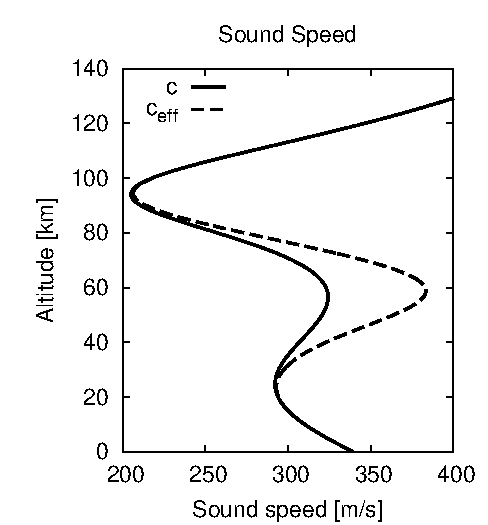
\includegraphics[scale=0.62]{figs/model_atmos_c}
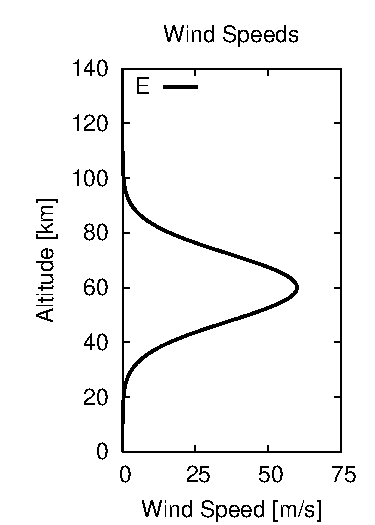
\includegraphics[scale=0.62]{figs/model_atmos_winds_u}
\end{center}
\caption{The NCPA model atmosphere, the ``toy'' model. The figure on the left shows sound speeds: the solid curve is the adiabatic sound speed and the dashed curve is the effective sound speed profile in the azimuth direction of 90 degrees (clockwise from North). The figure on the right shows the model zonal wind speed. The meridional wind speed is taken to be zero. The figures are taken from \cite{waxler2015stratospheric}.}
\label{fig:canonic_sound_speeds}
\end{figure}

To model propagation through a stratified medium only a single specification file is required. Range dependent profiles are specified by providing a directory of atmospheric specification files. In addition, the reading of G2S binary files is supported; however, there is no guarantee that the structure of the G2S binary files will remain unchanged. 